\documentclass[10pt,a4paper]{article}
\usepackage[margin=23mm]{geometry}
\usepackage[T1]{fontenc}
\usepackage{lmodern,microtype,amsmath,amssymb,booktabs,graphicx}
\usepackage[hidelinks]{hyperref}
\setlength{\parindent}{0pt}
\setlength{\parskip}{5pt}
\newcommand{\E}{\mathbb E}
\newcommand{\R}{\mathbb R}
\newcommand{\RiskRatio}{18.92}
\newcommand{\NativeError}{6.66e-16}
\newcommand{\EquilibriumError}{4.90e-16}
\newcommand{\NormError}{2.22e-16}
\newcommand{\CalibratedMC}{0.82363}
\newcommand{\CalibratedSE}{0.00670}
\newcommand{\BiasObserved}{0.00635}
\newcommand{\BiasExpected}{0.00646}

\title{JointGuard: dependence diagnostics for\protect\\ probabilistic elastic-response predictions}
\author{}
\date{20 October 2026}
\begin{document}
\maketitle
\vspace{-8mm}
\begin{abstract}
Can correct displacement marginals conceal a wrong prediction of spring stress?
An original two-degree-of-freedom elastic example isolates this question with
Gaussian response forecasts. We compare marginal continuous ranked probability
scores, joint logarithmic and energy scores, and a first-order variogram score.
Population expectations are evaluated analytically or by one-dimensional
quadrature, while a C++17 ensemble scorer is checked independently. An
independence approximation preserves every displacement marginal but predicts
an absolute stress exceedance probability \RiskRatio{} times the declared
truth. Conversely, a common displacement bias leaves both the variogram score
and central-spring stress risk unchanged. A finite-ensemble experiment separates
sampling variability from numerical error. The study provides reproducible
diagnostics for a synthetic model, not experimental validation or a new scoring rule.
\end{abstract}

\section{Question and mechanical model}
Probabilistic scientific models often produce joint predictions of spatial
responses. Marginal diagnostics do not determine the dependence between those
responses. This study asks whether that omission matters for a simple internal
force, and whether a dependence-sensitive score alone is sufficient. Proper
scoring rules supply a principled loss framework \cite{gneiting}; variogram
scores provide a complementary view of dependence \cite{scheuerer}.

Consider two axial displacements $u=(u_1,u_2)^T$, each connected to ground by
a spring and connected to each other by a third spring. All stiffnesses are
$k=10^6\,\mathrm{N/m}$. Quasi-static, small-displacement, linear equilibrium is
\begin{equation}
 K u=f,\qquad K=k\begin{bmatrix}2&-1\\-1&2\end{bmatrix},\qquad
 f\sim\mathcal N(0,\Sigma_f),\quad
 \Sigma_f=K(s^2 C_{0.9})K^T,\quad
 C_\rho=\begin{bmatrix}1&\rho\\\rho&1\end{bmatrix},
 \label{eq:mechanics}
\end{equation}
where $s=10^{-3}\,\mathrm m$. This deliberately prescribed load covariance
produces the dimensionless truth $Y=u/s\sim\mathcal N(0,C_{0.9})$.
The central-spring force is $k(u_2-u_1)$. Assigning a nominal cross-sectional
area $A=10^{-4}\,\mathrm{m^2}$ defines a stress proxy
$\sigma=k s(Y_2-Y_1)/A$. The event $|\sigma|>10\,\mathrm{MPa}$ is precisely
$|Y_2-Y_1|>1$. This is a chosen reporting threshold, not a measured yield limit.
For $D=a^TX$, $a=(-1,1)^T$, under any Gaussian forecast,
\begin{equation}
 P(|D|>b)=\Phi\!\left(\frac{-b-\mu_D}{s_D}\right)
             +\Phi\!\left(\frac{\mu_D-b}{s_D}\right),\qquad
 \mu_D=a^T\mu,\quad s_D^2=a^T\Sigma a. \label{eq:risk}
\end{equation}
No temporal integration, mesh or fitted parameter is involved. All scores use
the same fixed dimensionless displacement scale; their magnitudes cannot be
compared as if they had identical units or normalization.

\section{Scoring and numerical algorithm}
Let $F$ be the forecast law, $X,X'\sim F$ independent and $y$ an observed
response. Losses are oriented so that lower is better. The marginal score is
the average of two univariate CRPS values. Joint scores are
\begin{align}
 \operatorname{LogS}(F,y)&=-\log f_F(y),\\
 \operatorname{ES}(F,y)&=\E\|X-y\|_2-\tfrac12\E\|X-X'\|_2, \label{eq:es}\\
 \operatorname{VS}(F,y)&=(|y_1-y_2|-\E|X_1-X_2|)^2. \label{eq:vs}
\end{align}
The library generalizes VS to the average over unordered coordinate pairs
(order one, equal weights). Uniform shifts of the forecast cancel in each
pairwise difference, so VS is not strictly proper for the full joint law.
ES remains sensitive to dependence in population; this work does not label it
blind merely because its excess loss is smaller than another score's.

For $M$ independent ensemble members, the C++ implementation evaluates
\begin{equation}
 \widehat{\operatorname{ES}}_U=
 \frac1M\sum_{i=1}^M\|x_i-y\|_2-
 \frac{1}{M(M-1)}\sum_{i<j}\|x_i-x_j\|_2. \label{eq:ensemble}
\end{equation}
This estimates the population score without finite-ensemble bias when members
are iid and independent of $y$. Replacing $M(M-1)$ by $M^2$ instead computes
the score of the finite empirical distribution, with expected excess
$\E\|X-X'\|_2/(2M)$ over the population score. Neither denominator is universally
correct: it depends on which distribution is being evaluated. The iid correction
is not justified for correlated ensemble members.

For independent Gaussian forecast and truth, the two norms in the population
ES have Gaussian arguments. For $Z\sim\mathcal N(m,S)$, define
\begin{equation}
 L(t)=\E e^{-tZ^TZ}=
 \frac{\exp[-t m^T(I+2tS)^{-1}m]}{\sqrt{\det(I+2tS)}}.
 \qquad
 \E\|Z\|_2=\frac1{\sqrt\pi}\int_0^\infty
             \frac{1-L(x^2)}{x^2}\,dx. \label{eq:quad}
\end{equation}
The integral follows by applying the Laplace representation of $\sqrt z$ to
$Z^TZ$ and substituting $t=x^2$. We diagonalize $S$, normalize the scale,
use \texttt{log1p}/\texttt{expm1} to avoid subtraction cancellation, and apply
adaptive quadrature with absolute and relative tolerances $2\times10^{-11}$
in normalized units. Its error estimate is not a rigorous certificate.

Closed-form folded-normal moments give $\E|Z|$ and therefore population CRPS
and VS. Gaussian expected LogS follows from a trace term, a squared mean-error
term and a log determinant. Cholesky solves avoid explicit covariance inverses.
Force moments propagate as $\mu_u=K^{-1}\mu_f$ and
$\Sigma_u=K^{-1}\Sigma_f K^{-T}$. Inputs must be finite with symmetric
positive-definite covariance and stiffness; singular laws are not supported.

\section{Implementation and reproducible experiment}
The repository contains a C++17 distance core, pybind11 bindings, and a Python
package for Gaussian diagnostics, elastic propagation and experiments.
For $N$ observations in $d$ dimensions, the native scorer costs
$O((M^2+NM)d)$ operations and $O(N)$ auxiliary storage; it does not allocate
a pairwise distance matrix. No measured runtime speedup is claimed.

Four forecasts are specified without training: calibrated $\mathcal N(0,C_{0.9})$,
independent $\mathcal N(0,I)$, anticorrelated $\mathcal N(0,C_{-0.5})$, and
common bias $\mathcal N((1,1)^T,C_{0.9})$. A 64-point correlation sweep on
$[-0.9,0.99]$ retains unit marginal variances. The stochastic check uses
NumPy's default random generator with seed 20261020, 24 independent replicates,
128 ensemble members and 256 independent observations per replicate. Within
each replicate the candidates share latent Gaussian draws for paired comparison;
observations and forecast ensembles are independent. Standard errors are computed
across replicate means and include both ensemble and observation sampling.

The command \texttt{jointguard --output results} regenerates the experiment.

Run \texttt{scripts/check\_results.py} with Python for an independent repeat.
JSON metrics, three CSV tables, the figure, and LaTeX tables/macros share this experiment.
The paper imports these artifacts directly. The build script rejects unresolved
references, overfull boxes and more than five pages, and records SHA-256 hashes
of every paper input and the PDF. CI tests Windows and Ubuntu builds and
independently compiles the paper with pdfLaTeX.

\section{Results and validation}
\begin{table}[ht]
\centering
\begin{tabular}{lrrrrr}
\toprule
Forecast & CRPS & LogS & ES & VS & Risk (\%) \\
\midrule
Calibrated & 0.5642 & 2.0075 & 0.8267 & 0.0727 & 2.535 \\
Independent & 0.5642 & 2.8379 & 0.8626 & 0.6680 & 47.950 \\
Anticorrelated & 0.5642 & 3.6274 & 0.8965 & 1.1236 & 56.370 \\
Common bias & 0.8351 & 2.5338 & 1.2049 & 0.0727 & 2.535 \\
\bottomrule
\end{tabular}

\caption{Expected loss under the declared truth, and forecast probability of
absolute stress exceedance. ES uses deterministic quadrature; all other columns
are closed form. Values are generated, not estimates from the finite sample.}
\label{tab:population}
\end{table}
Table~\ref{tab:population} shows that the three zero-mean forecasts have
identical marginal CRPS, despite substantially different extension risk.
Ignoring the positive response correlation raises the predicted exceedance
probability by a factor of \RiskRatio. Joint LogS, ES and VS each identify
this dependence error in population. A uniform mean shift instead leaves VS
and central-spring risk unchanged while increasing marginal CRPS, LogS and ES.
Being irrelevant to this particular stress event does not make that bias
irrelevant to displacement predictions or the two grounding-spring forces.

\begin{figure}[ht]
\centering
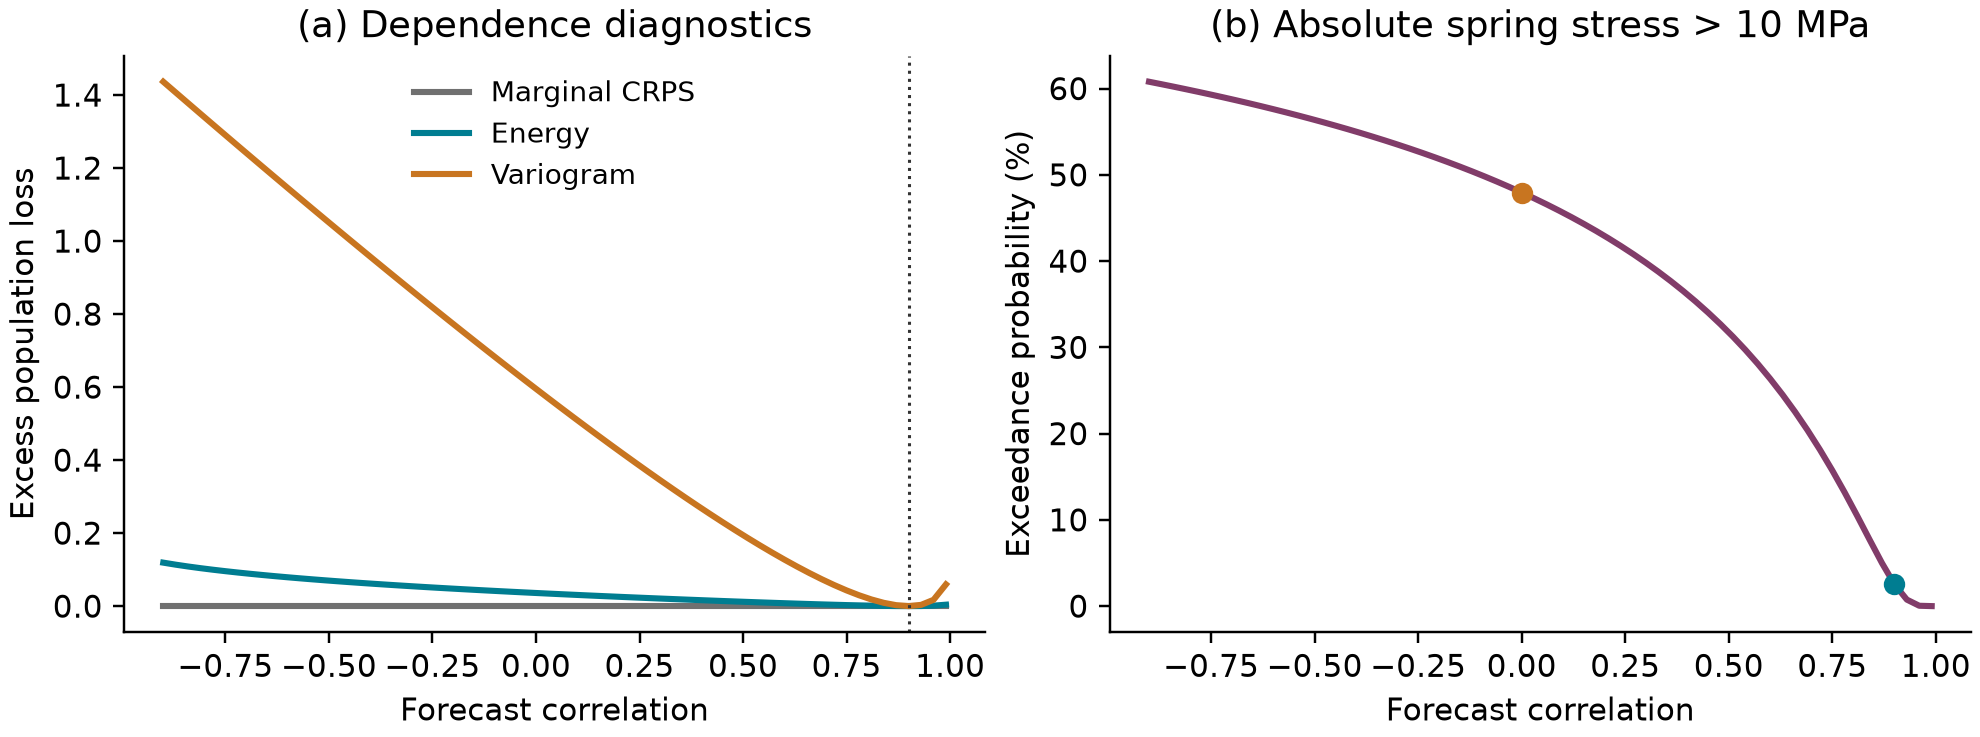
\includegraphics[width=\linewidth]{../results/joint-study.png}
\caption{Original correlation sweep. (a) Excess loss relative to the calibrated
forecast; the dotted line marks true correlation. Different losses have different
scales, so their vertical separation is not a universal sensitivity ranking.
(b) Predicted absolute stress exceedance; dots mark calibrated and independent
forecasts. Marginals stay unchanged throughout the sweep.}
\label{fig:sweep}
\end{figure}

For the calibrated forecast, the finite-ensemble mean unbiased ES is
\CalibratedMC{} with replicate standard error \CalibratedSE{}, compared with
population ES in Table~\ref{tab:population}. The observed empirical-minus-unbiased
difference is \BiasObserved{}, versus expected bias \BiasExpected{} for $M=128$.
These are finite-sample results, not quadrature errors; the 24-replicate standard
error is itself estimated. The reproduction check requires each model's ensemble
mean to fall within four estimated standard errors of its population ES. This
fixed-seed regression check does not establish a general confidence guarantee.

Independent numerical checks compare native scores against SciPy distance
matrices (maximum absolute error \texttt{\NativeError}), verify the equilibrium
covariance identity (relative Frobenius residual \texttt{\EquilibriumError}),
and compare the isotropic two-dimensional norm with its Rayleigh mean
(absolute error \texttt{\NormError}). These are roundoff-scale observations,
not claims of portable last-digit accuracy. Tests additionally cover
noncentral one-dimensional norm quadrature, chi-distribution means, Gaussian
log densities, invariance properties, input rejection and native overflow.

\section{Discussion, limitations and conclusion}
This example separates three questions. \emph{Discrete implementation error}
is checked by algebraic identities and independent distance calculations.
\emph{Numerical integration error} enters population ES through quadrature;
the other population values are closed form. \emph{Continuum error} is not
estimated: the three-spring model is the stipulated discrete system, and no
continuum discretization or mesh-convergence claim is made. Sampling uncertainty
is reported separately for finite ensembles. None of these tests establishes
\emph{physical validity}; no measured material data, nonlinear constitutive
response, inertia, failure model or experimental stress observations are used.

The findings apply to fixed, nonsingular Gaussian laws in a common coordinate
scale. Non-Gaussian, high-dimensional, time-dependent and data-fitted forecasts
could behave differently. The stress threshold illustrates a decision-relevant
quantity but does not define a design safety assessment. Score comparisons alone
do not supply tail calibration, and numerical loss magnitudes cannot be ranked
across score families without considering their scales and targets.

The reproducible result is a complementary diagnostic workflow: assess marginals,
evaluate the joint law, and inspect the actual mechanical functional of interest.
Correct marginals can conceal large extension-risk errors, while a variogram
can conceal a common displacement bias. Neither diagnostic should be used alone.
The project was motivated by DTU ATSA lecture topics on multivariate forecast
evaluation; no private course material is redistributed.

\begin{thebibliography}{9}
\bibitem{gneiting} T. Gneiting and A. E. Raftery.
Strictly proper scoring rules, prediction, and estimation.
\emph{Journal of the American Statistical Association}, 102(477):359--378, 2007.
\href{https://doi.org/10.1198/016214506000001437}{doi:10.1198/016214506000001437}.
\bibitem{scheuerer} M. Scheuerer and T. M. Hamill.
Variogram-based proper scoring rules for probabilistic forecasts of multivariate quantities.
\emph{Monthly Weather Review}, 143(4):1321--1334, 2015.
\href{https://doi.org/10.1175/MWR-D-14-00269.1}{doi:10.1175/MWR-D-14-00269.1}.
\end{thebibliography}
\end{document}
